\section{Machine Learning Applied to a BSM Search}\label{sec:MLHEP}
So far I have presented the goal of my analysis (to discover new physics)
as well as the tools I will be using to achieve it (\ac{ML}). In this section
I will discuss how \ac{ML} is applied to the problem as well as how it compares
to traditional methods.
\subsection{The Traditional Approach}
As discussed, I have been presented with two sets of data; the measured collision 
data from \ac{ATLAS} and the simulated \ac{MC} data. The origin of the latter data set 
will not be covered in great detail in this thesis, but it is worth mentioning that 
the simulations are based on \ac{SM} theory. In other words, by comparing the measured collision 
data with the \ac{SM} simulations, we are essentially comparing what is predicted by the \ac{SM} 
to what is measured by experiment. If the two differ in ways not explained by simulation inadequacies or
features of the data that are unrelated to physics, one could interpret the deviation 
as new physics.
\\
In short, a search for new physics, is a search for deviations in the comparisons of simulations 
to experimental data. At first thought, this might seem like a simple task. Given that the deviations 
would be large, it would be easy. In reality, any new physics predicting large contributions 
in the data currently measured by \ac{ATLAS} has been excluded a long time ago. Today, any
promising extension of the \ac{SM} predicts to contribute rarely in any collision. As will 
be presented in later sections some theories that will be searched for in this thesis only 
contribute to a total of 6 collisions in a data set consisting of more than $3800000$ events 
($<0.002\%$). Not only would such a deviation be incredibly hard to detect, but it would 
be close to impossible to determine if such a deviation is rooted in new physics or statistical fluctuations 
of the background. 
\\
The traditional approach to this problem is to study the data in physics motivated regions. 
For example, in section \ref{sec:signal} I presented the Feynman diagrams of the \ac{SUSY} signals I 
searched for in this thesis. As mentioned, this type of final state is expected to exhibit 
large amounts of missing transverse energy\footnote{Due to the neutralinos being both heavy, neutral 
and interacting only weakly with ordinary matter.}. The traditional approach is to neglect all the data 
with small amounts of missing energy, and only consider events of interest. By applying these kinds of 
constraints on the data, you are creating a region where you expect to find as much of the signal and as little 
of the background as possible. After applying a sufficient amount of demands (or cuts), you would count the 
remaining data in your \emph{search region} and check for deviation. This approach is called \acf{CC}.
\\
\begin{figure} 
    \centering
    \makebox[0.75\linewidth][c]{%
    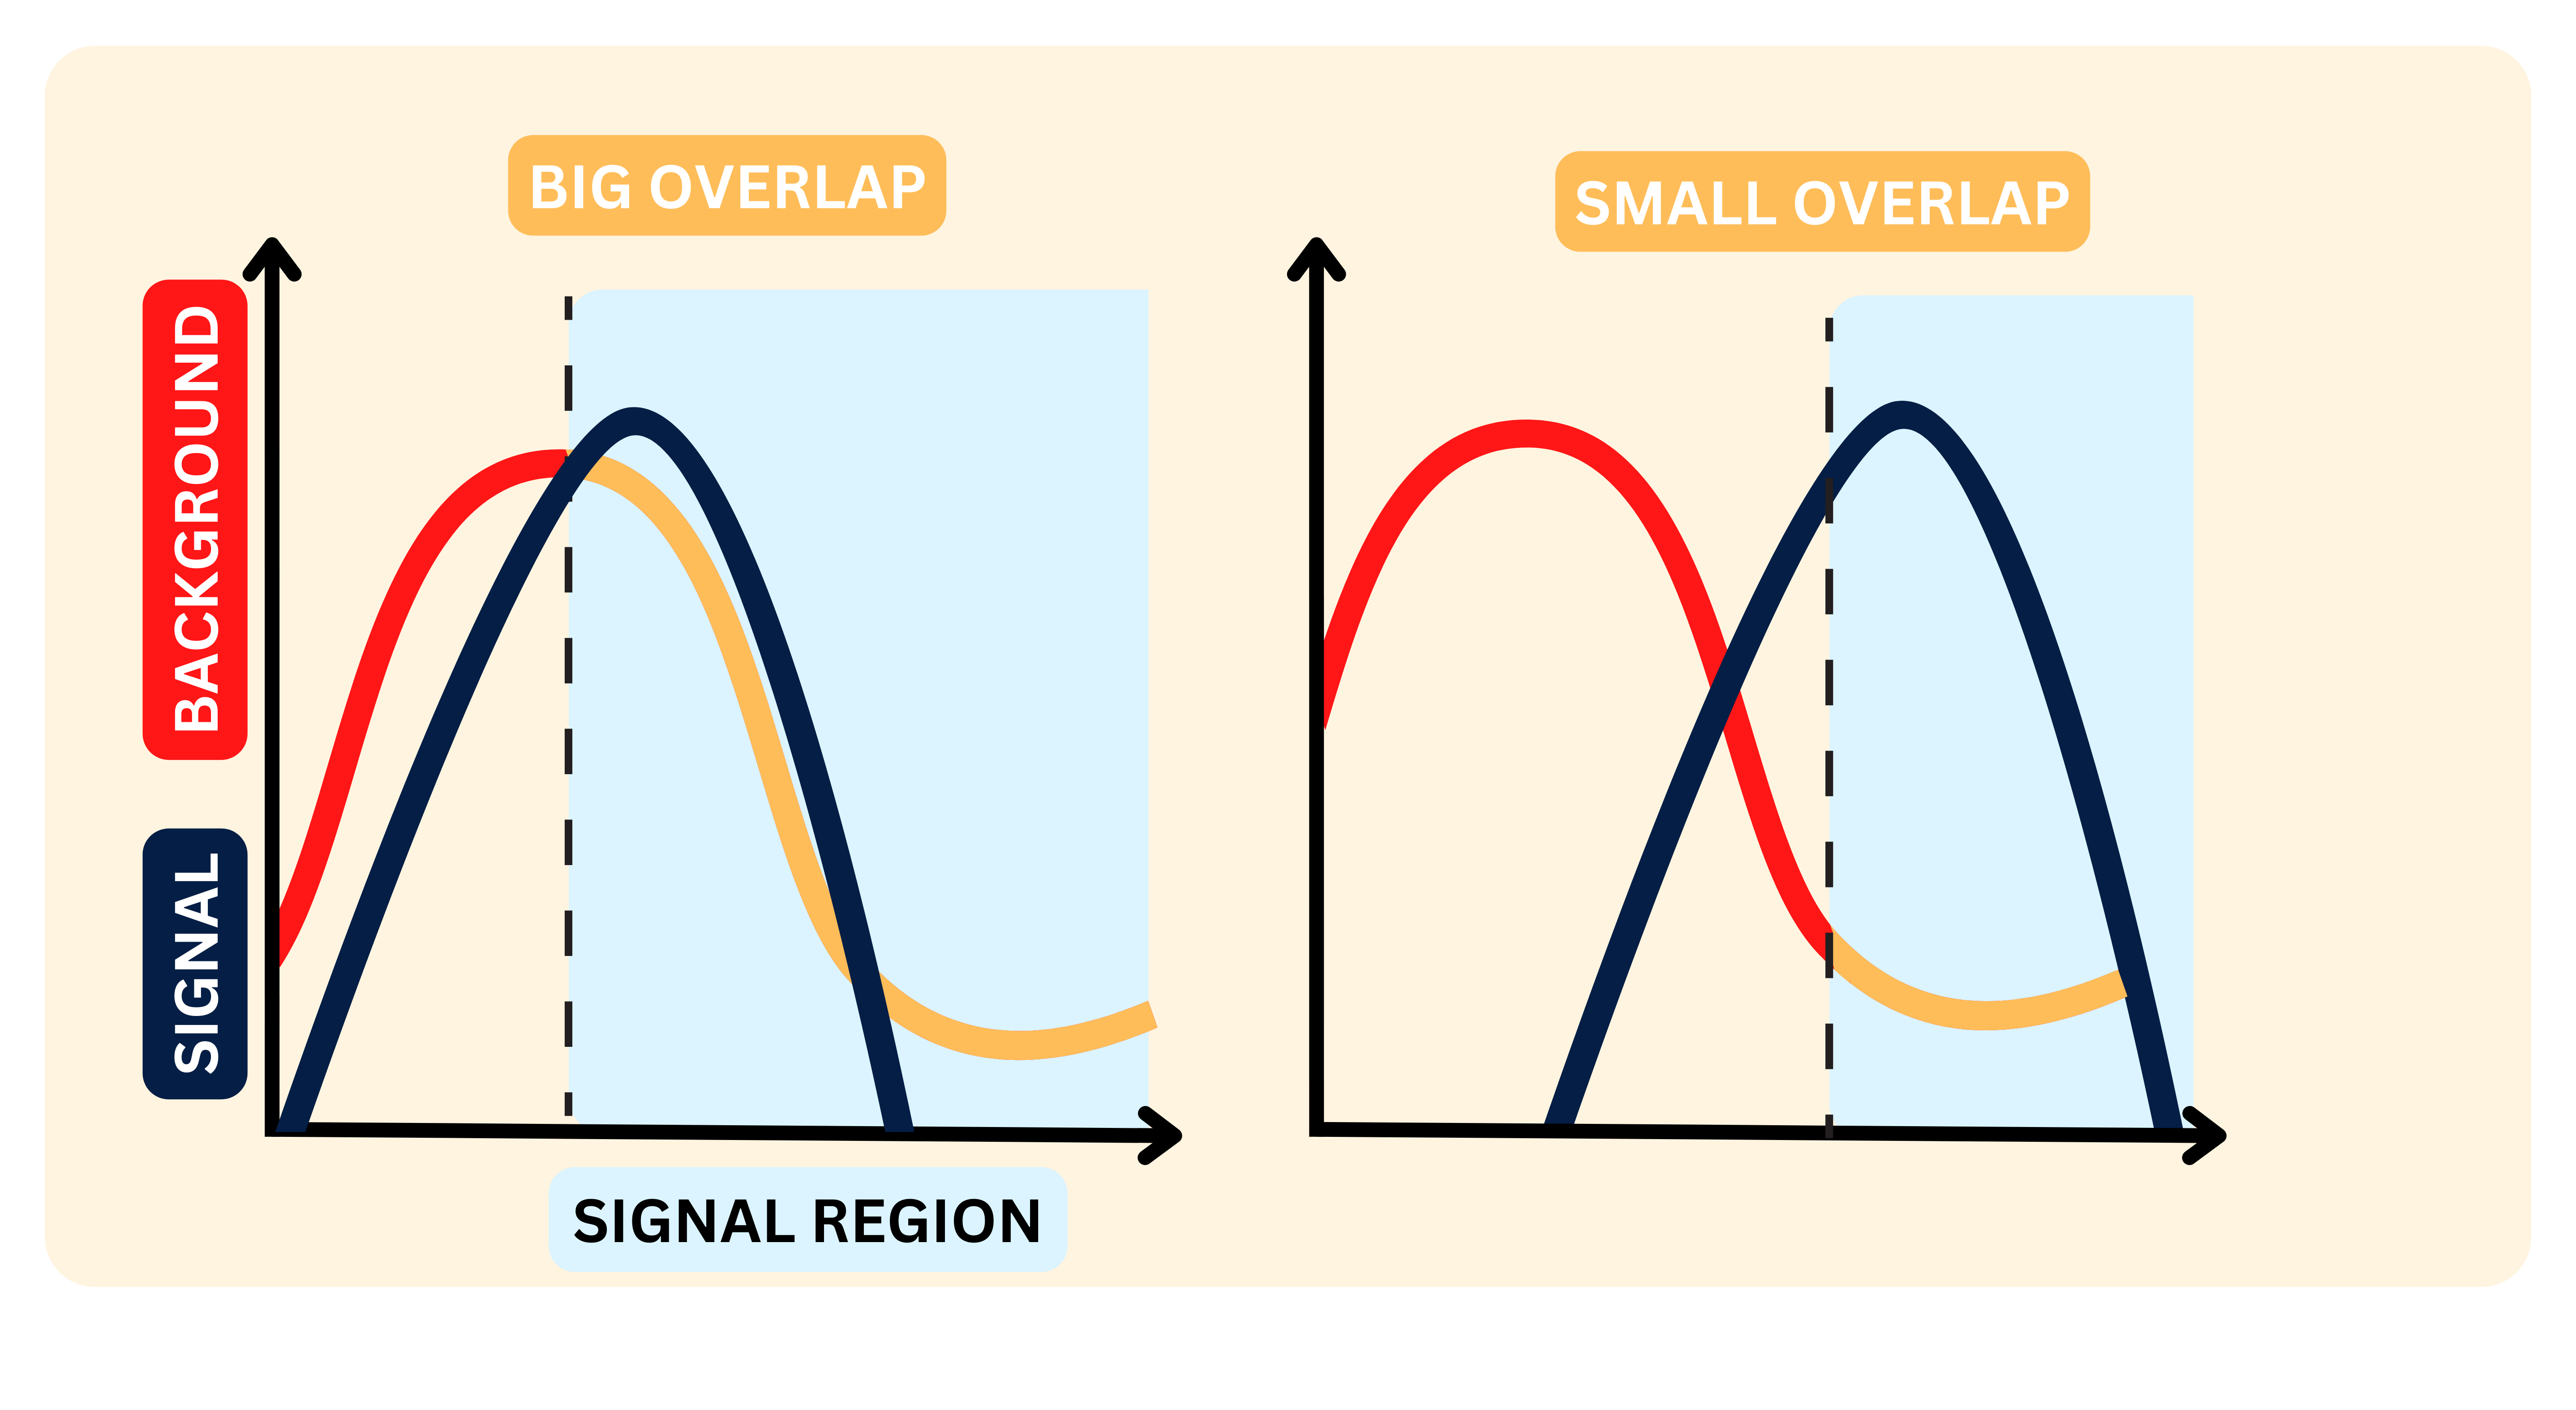
\includegraphics[width=0.65\textwidth]{Figures/Illustrations/CandC.png}
    }
    \caption[An illustration of a traditional \acs{CC} approach and how non-overlapping features lead to effective
    signal regions.]{An illustration of a traditional \acf{CC} approach and how non-overlapping features lead to effective
    signal regions. In the first figure (left) the distributions of signal and background are relatively similar, and 
    the signal region contains large amounts of background. In the second (right), the distributions of signal and 
    background are greatly different, and this variable would allow for a much more effective signal region. }
    \label{fig:overlap}
\end{figure}
\subsection{The Machine Learning Approach}
For a signal which greatly differs from the \ac{SM}, the \ac{CC} method could be sufficient. But, in 
cases where the signal is similar to background, it becomes harder to create effective\footnote{By effective
cuts I mean cuts which remove large amounts of the background while at the same time preserve as much of 
the signal as possible.} cuts. In figure \ref{fig:overlap}, I have drawn an illustration of two different feature distributions both 
displaying the distribution for a hypothetical signal and background. Additionally, I have drawn a 
threshold in both distributions which represents the cut made to create a search region. In the first 
figure (left) the distributions of signal and background are relatively similar, and the signal region 
contains large amounts of background. In the second (right), the distributions of signal and background 
are greatly different, and this variable would allow for a much more effective signal region. 
\\
The goal of introducing \ac{ML}, is to create a new feature in the data set where background and signal
exhibit as little overlap as possible. This is very similar to how we introduce physics motivated high-level
features like invariant mass, but instead of using an analytical function grounded in physics, 
we apply the output of a trained \ac{ML} model. Then, once the \ac{ML}-variable is created, 
we apply a cut (similar to \ac{CC}) which will define an effective search region. 
\\
How we create the \ac{ML}-variable can vary depending on the type of \ac{ML}. An effective unsupervised approach
would be incredibly beneficial, as it would be totally model independent. In other words, the same model could be applied 
to all signal. As mentioned in earlier sections (see section \ref{sec:MLPhen}), the focus of this thesis will not be on 
unsupervised \ac{ML}, but supervised. The largest difference between the two is the introduction of an additional data set,
the simulated signal. By training on the simulated signal, we are able to achieve a much more 
effective output which is tailored to what we expect the new physics to look like. Though, what supervised learning gains in performance
it loses in generalizability, i.e. the ability to find new physics it has not trained on.